% Copyright 2013 Nicolai Hähnle <nhaehnle@gmail.com>
%
% This work is licensed under the Creative Commons Attribution-ShareAlike 3.0
% Unported License, see http://creativecommons.org/licenses/by-sa/3.0/
%
% Among other things, this means that yes, you may take e.g. illustrations from
% the book and use them in your own work. However, (a) you must give proper
% attribution by naming me as its original author and (b) you must make your
% derivative work available under the same or similar license terms.
%
% See the Creative Commons website for the exact licensing terms.

\chapter{Generating Functions and the Algebra of Polyhedra}

We have seen how to enumerate the lattice points in a convex body $K$
in time that is essentially proportional to the maximum number of lattice points
in a translate of $K$.
What if we are only interested in the \emph{number} $|K \cap \Lambda|$ of such points?

Throughout this chapter, we will work with $\Lambda = \Z^d$ -- using a linear transformation,
this is without loss of generality.
Consider the box $K = [0,M]^d$.
It contains roughly $M^d$ integer points, which is exponential in the number of bits
required to encode a description of $K$.
On the other hand, computing this number is a trivial task that can be performed in
polynomial time in the encoding length of $K$.
This leads us to suspect that \emph{computing the number} of integer points could be
exponentially faster than \emph{enumerating} all those points.

In the case of a box,
computing the number of points is a polynomial problem even when the dimension $d$ is allowed to vary.
We do not expect this to be true in general
because the problem of deciding whether $|P \cap \Z^d|$ is $0$ for an arbitrary polytope $P$ is the integer programming problem,
which is $NP$-hard.
In fact, computing $|P \cap \Z^d|$ is easily seen to be a $\# P$-hard problem.
So we should contend ourselves with looking for an algorithm that is polynomial so long as $d$ is fixed,
and with trying to reduce the dependence on $d$ of the degree of this polynomial.

The enumeration algorithms of the last chapter could be formulated with representations of convex bodies via oracles.
This is no longer the case for computing the number of integer points.
Let $N \in \N$ and consider the convex body
\[
  K_\varepsilon(a,b) := \{ (x,y) \in \R^2 ~:~ a \leq x \leq b, xy \geq N + \varepsilon, y \leq N \}
\]
The lower envelope of $K_0(a, b)$ contains an integer point if and only if $N$ has a factor between $a$ and $b$,
see Figure~\ref{fig:factoring-body}.
Consequently, for $\varepsilon \in (0,1)$ one has $|K_0 \cap \Z^2| - |K_\varepsilon \cap \Z^2| > 0$ if and only if $N$ has a factor between $a$ and $b$.
\begin{fact}
  If there were a polynomial-time algorithm for computing the number of integer points in (somewhat general) convex bodies in $\R^2$,
  then one could factor integers in polynomial time.
\end{fact}
We don't expect factoring to be a polynomial time problem,
so we cannot hope to count integer points in arbitrary convex bodies.
Instead, our goal will be a polynomial time algorithm that counts the number of integer points in \emph{polytopes}
in fixed dimension.

\begin{figure}
  \begin{center}
    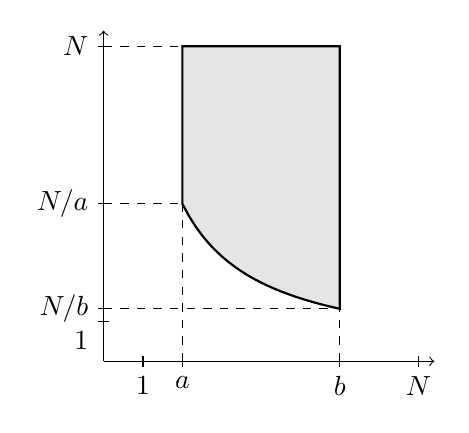
\begin{tikzpicture}
      \draw[->] (0,0) -- (4.2,0);
      \draw[->] (0,0) -- (0,4.2);
      
      \draw[dashed] (0,0.666) -- (3,0.666);
      \draw[dashed] (0,2) -- (1,2);
      \draw[dashed] (0,4) -- (1,4);
      
      \draw[dashed] (1,0) -- (1,2);
      \draw[dashed] (3,0) -- (3,0.666);

      \draw (0.5,0) +(0,2pt) -- +(0,-2pt) node[below] {$1$};
      \draw (1,0) +(0,2pt) -- +(0,-2pt) node[below] {$a$};
      \draw (3,0) +(0,2pt) -- +(0,-2pt) node[below] {$b$};
      \draw (4,0) +(0,2pt) -- +(0,-2pt) node[below] {$N$};
      \draw (0,0.5) +(2pt,0) -- +(-2pt,0) node[below left] {$1$};
      \draw (0,2) +(2pt,0) -- +(-2pt,0) node[left] {$N/a$};
      \draw (0,0.666) +(2pt,0) -- +(-2pt,0) node[left] {$N/b$};
      \draw (0,4) +(2pt,0) -- +(-2pt,0) node[left] {$N$};
      
      \draw[thick,fill=black!10] plot[domain=1:3] (\x, {2 / \x}) -- (3,4) -- (1,4) -- cycle;
    \end{tikzpicture}
  \end{center}
  \caption{The body $K_0(a,b)$ encodes information about the factors of $N$.}
  \label{fig:factoring-body}
\end{figure}



\section{A simple example of generating functions}
\label{sec:simple-example-generating-functions}

Suppose we want to count the number of integer points in an interval $I := [a,b] \subset \R$
in a way that might be extendable to higher dimension.
One way of doing this is to symbolically determine the \emph{generating function}
\[
  f(I;x) = \sum_{p \in I \cap \Z} x^p
\]
and evaluate it at the point $f(I;1) = |I \cap \Z|$.
Unfortunately, $f(I;x)$ is the sum of $|I \cap \Z|$ monomials.
The memory space required for writing this sum down is therefore exponential in the encoding length of $I$.
A better approach is needed. The geometric series
\[
  \sum_{p = 0}^\infty x^p
\]
is at the same time the generating function for the unbounded interval $[0,\infty)$
and satisfies
\[
  \sum_{p = 0}^\infty x^p = \frac{1}{1 - x}
\]
where the series converges absolutely.
The following picture suggest a way to leverage the geometric series for our problem:
\begin{center}
  \begin{tikzpicture}
    \draw (-0.2,0) -- (8.2,0);
    \foreach \x in {0,0.5,...,8.01}
      \draw (\x,0) +(0,2pt) -- +(0,-2pt);
    
    \draw[very thick] (2,0) node[below] {$a$} -- node[above] {$I$} (5,0) node[below] {$b$};
    
    \draw (2,-1) +(0,2pt) -- +(0,-2pt) +(0,0) -- (8.2,-1);
    \draw (5.5,-1.5) +(0,2pt) -- +(0,-2pt) +(0,0) -- (8.2,-1.5);
    
    \draw (1,-1) node {$=$};
    \draw (1,-1.5) node {$-$};
  \end{tikzpicture}
\end{center}
The graphical ``formula'' carries over to formal Laurent series (assuming $a, b \in \Z$ for simplicity):
\[
  \sum_{p = a}^b x^p = \sum_{p = a}^\infty x^p - \sum_{p = b+1}^\infty x^p
\]
There is an open set $U \subset \C$ on which all series converge absolutely,
and so
\[
  \sum_{p = a}^b x^p = \frac{x^a}{1 - x} - \frac{x^{b + 1}}{1 - x}
\]
holds on $U$.
Since the functions involved in this equation are rational and therefore complex differentiable,
it follows that the equality must hold on all of $\C$ (except for $x = 1$, where the functions are not defined).
That is, we can write
\[
  f(I;x) = \frac{x^a}{1 - x} - \frac{x^{b + 1}}{1 - x}
\]
if we understand the equality to be up to negligible differences in the domains of the two sides of the equation.
Observe that the encoding length of the right hand side is dominated by the encodings of $a$ and $b$,
and is therefore linear in the encoding length of $I$.

The downside of this representation of $f(I;x)$ is that it is undefined at $x = 1$,
which is exactly the point where we would like to evaluate it.
However, $x = 1$ is a removable singularity.
Using the rule of de~l'Hôpital, we can compute
\[
  \lim_{x \to 1} \frac{x^a}{1 - x} - \frac{x^{b + 1}}{1 - x} = \lim_{x \to 1} \frac{x^a - x^{b+1}}{1 - x} = \lim_{x \to 1} \frac{a x^{a-1} - (b+1) x^b}{-1} = b - a + 1,
\]
which is the correct answer, as the derivation above has already shown.

Note that the graphical formula we used to derive the rational generating function for $I$ is by no means unique.
The following picture shows an alternative formula:
\begin{center}
  \begin{tikzpicture}
    \draw (-0.2,0) -- (8.2,0);
    \foreach \x in {0,0.5,...,8.01}
      \draw (\x,0) +(0,2pt) -- +(0,-2pt);
    
    \draw[very thick] (2,0) node[below] {$a$} -- node[above] {$I$} (5,0) node[below] {$b$};
    
    \draw (2,-1) +(0,2pt) -- +(0,-2pt) +(0,0) -- (8.2,-1);
    \draw (-0.2,-1.5) -- (5,-1.5)  +(0,2pt) -- +(0,-2pt);
    \draw (-0.2,-2) -- (8.2,-2);
    
    \draw (-1,-1) node {$=$};
    \draw (-1,-1.5) node {$+$};
    \draw (-1,-2) node {$-$};
  \end{tikzpicture}
\end{center}
Again, this carries over to formal Laurent series:
\[
  \sum_{p = a}^b x^p = \sum_{p = a}^\infty x^p + \sum_{p = -\infty}^b x^p - \sum_{p = -\infty}^\infty x^p
\]
There are two problems:
\begin{itemize}
  \item The first two series on the right hand side are geometric series for which a rational function expression is known.
    However, their regions of absolute convergence are disjoint.
  
  \item The last series does not converge anywhere, and it is unclear what rational function expression could be used in its place.
\end{itemize}
Over the course of this chapter,
we will see that the first problem turns out not to be a problem after all,
and that the last, non-converging series, magically disappears.
One finds that
\[
  f(I;x) = \frac{x^a}{1-x} + \frac{x^b}{1-x^{-1}}
\]
where, again, the equality should be understood modulo negligible differences in the functions' domains.
For now, the reader may want to convince themselves that the equation holds in this particular example,
for example by manual comparison to the rational function obtained previously.

The remainder of this chapter generalizes the approach we have just laid out to higher dimension,
exploring some rather fascinating algebraic structures on the way.



\section{Cones and triangulations}

\begin{definition}
  \begin{enumerate}[(a)]
    \item A non-empty convex set $K \subseteq \R^d$ is a \emph{cone}
      if $p \in K$ and $\lambda \geq 0$ imply $\lambda p \in K$.
  
    \item A \emph{conic combination} of vectors $u_1, \ldots, u_n \in \R^d$ is
      a linear combination with non-negative coefficients.
  
    \item Given $U \subset \R^d$, the set $\cone(U)$ is the set of conic combinations of vectors in $U$.
  
    \item A cone $K$ is \emph{polyhedral} if $K$ is a polyhedron.
  \end{enumerate}
\end{definition}

Note that cones are closed under taking conic combinations,
and $\cone{U}$ is the smallest cone containing $U$.

\begin{definition}
  Let $P$ be a non-empty polyhedron.
  The \emph{lineality space} of $P$ is
  \[
    L(P) := \{ v \in \R^d ~:~ \forall x\in P \,\forall \lambda \in \R:~ x + \lambda v \in P  \}
  \]
  If $L(P) = 0$, $P$ is called \emph{pointed}.
\end{definition}

It is not difficult to check that $L(P)$ is a linear subspace of $\R^d$.
Intuitively, $L(P)$ contains the directions of lines contained in $P$.
Polyhedra containing lines are somewhat unusual in the sense
that if one thinks of polyhedra, one usually thinks of polyhedra that have vertices,
and such polyhedra \emph{do not} contain lines.
That is, their lineality space is $0$.
However, their properties are crucial for the development of compact rational generating functions.

The following facts tie cones, polarity, and lineality spaces together.
Their proofs are left as an exercise.

\begin{lemma}
  \label{lemma:cone-polars}
  Let $K \subseteq \R^d$ be a closed cone.
  \begin{enumerate}[(a)]
    \item $K^\star = \{ y \in \R^d ~:~ y^Tx \leq 0 \,\forall\, x\in K \}$.
    \item $K^\star$ is a cone and $(K^\star)^\star = K$.
    \item $d = \dim L(K) + \dim K^\star$.
  \end{enumerate}
\end{lemma}

\begin{definition}
  A cone $K$ is \emph{simplicial} if $K = \cone\{ u_1, \ldots, u_k \}$ for linearly independent vectors $u_j \in \R^d$.
\end{definition}

\begin{definition}
  Let $K \subset \R^d$ be a full-dimensional simplicial cone,
  $K = \cone\{ u_1, \ldots, u_d \}$
  with $u_j \in \Z^d$ primitive integer vectors.
  Then the \emph{determinant} of $K$ is
  \[
    \det(K) := |\det(u_1,\ldots,u_d)|
  \]
  A \emph{unimodular} cone is a full-dimensional simplicial cone with determinant $1$.
\end{definition}

Again, the proofs of the following facts about simplicial and unimodular cones are left as an exercise.

\begin{lemma}
  \label{lemma:simplicial-cone-polars}
  Let $K = \cone\{u_1,\ldots,u_d\} \subset \R^d$ be a full-dimensional simplicial cone.
  \begin{enumerate}[(a)]
    \item Let $A = (u_1, \ldots, u_d)$. Then $K = \{ p \in \R^d ~:~ -A^{-1} p \leq 0 \}$.
    \item $K^\star$ is simplicial.
    \item $K$ is unimodular if and only if $K^\star$ is unimodular.
  \end{enumerate}
\end{lemma}

\begin{figure}
  \begin{center}
    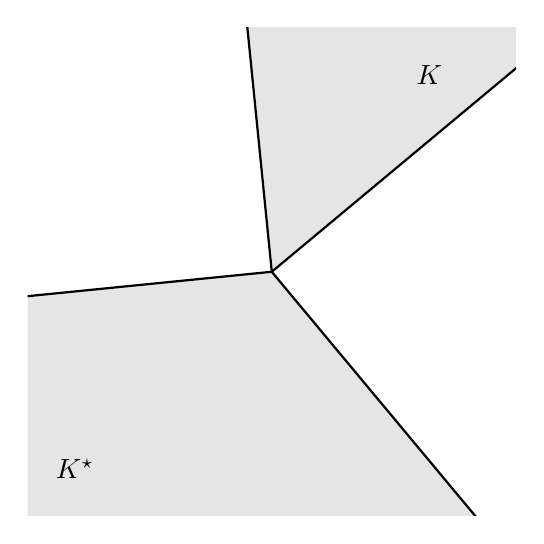
\begin{tikzpicture}
      \clip (-3.1,-3.1) rectangle (3.1,3.1);
      
      \draw[thick,fill=black!10] (-0.5,5) -- (0,0) -- (6,5);
      \draw[thick,fill=black!10] (-10,-1) -- (0,0) -- (10,-12);
      \draw (2,2.5) node {$K$};
      \draw (-2.5,-2.5) node {$K^\star$};
    \end{tikzpicture}
  \end{center}
  \caption{A simplicial cone and its polar.}
\end{figure}


Working with simplicial cones is desirable due to their simple combinatorial structure.
For this reason, we want to \emph{triangulate} more complicated polyhedral cones into simplicial cones.
We start by defining the notion of triangulation for polytopes,
see Figure~\ref{fig:triangulation-example}.

\begin{definition}
  Let $P \subset \R^d$ be a polytope.
  A set of simplices $\Delta_1, \ldots, \Delta_n$ is a \emph{triangulation} of $P$ if
  \begin{enumerate}
    \item $P = \bigcup_j \Delta_j$ and
    \item for every $i \neq j$, $\Delta_i \cap \Delta_j$ is a face of both $\Delta_i$ and $\Delta_j$ (possibly the empty face).
  \end{enumerate}
\end{definition}

\begin{figure}
  \begin{center}
    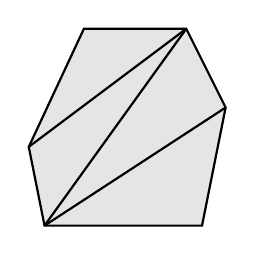
\begin{tikzpicture}
      \coordinate (n1) at (0,0);
      \coordinate (n2) at (2,0);
      \coordinate (n3) at (2.3,1.5);
      \coordinate (n4) at (1.8,2.5);
      \coordinate (n5) at (0.5,2.5);
      \coordinate (n6) at (-0.2,1);
      
      \draw[thick,fill=black!10] (n1) -- (n2) -- (n3) -- (n4) -- (n5) -- (n6) -- cycle;
      \draw[thick] (n1) -- (n3);
      \draw[thick] (n1) -- (n4);
      \draw[thick] (n4) -- (n6);
    \end{tikzpicture} \qquad
    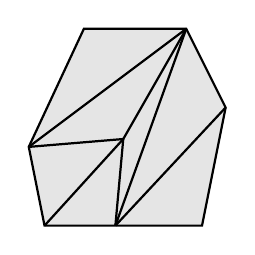
\begin{tikzpicture}
      \coordinate (n1) at (0,0);
      \coordinate (n2) at (2,0);
      \coordinate (n3) at (2.3,1.5);
      \coordinate (n4) at (1.8,2.5);
      \coordinate (n5) at (0.5,2.5);
      \coordinate (n6) at (-0.2,1);
      \coordinate (t0) at (0.9,0);
      \coordinate (t1) at (1,1.1);
      
      \draw[thick,fill=black!10] (n1) -- (n2) -- (n3) -- (n4) -- (n5) -- (n6) -- cycle;
      \draw[thick] (n1) -- (t1);
      \draw[thick] (n6) -- (t1);
      \draw[thick] (n4) -- (t1);
      \draw[thick] (t0) -- (n3);
      \draw[thick] (n4) -- (n6);
      \draw[thick] (t0) -- (t1);
      \draw[thick] (t0) -- (n4);
    \end{tikzpicture} \qquad
    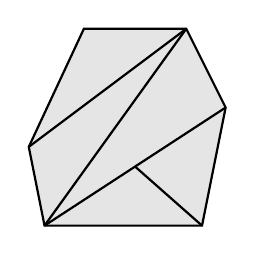
\begin{tikzpicture}
      \coordinate (n1) at (0,0);
      \coordinate (n2) at (2,0);
      \coordinate (n3) at (2.3,1.5);
      \coordinate (n4) at (1.8,2.5);
      \coordinate (n5) at (0.5,2.5);
      \coordinate (n6) at (-0.2,1);
      \coordinate (t0) at (1.15,0.75);
      
      \draw[thick,fill=black!10] (n1) -- (n2) -- (n3) -- (n4) -- (n5) -- (n6) -- cycle;
      \draw[thick] (n1) -- (n3);
      \draw[thick] (n1) -- (n4);
      \draw[thick] (n4) -- (n6);
      \draw[thick] (n2) -- (t0);
    \end{tikzpicture}
  \end{center}
  \caption{The first two pictures show triangulations. The last picture does not satisfy the second condition of the definition.}
  \label{fig:triangulation-example}
\end{figure}

\begin{theorem}
  \label{thm:polytope-triangulation}
  Let $P = \conv\{ v_1, \ldots, v_n \} \subset \R^d$ be a full-dimensional polytope.
  There is a triangulation $\Delta_1, \ldots, \Delta_m$ of $P$
  such that each simplex $\Delta_j$ is spanned by some subset of $d+1$ vectors from the set $\{ v_j \}_j$.

  If $P$ is rational, such a triangulation can be computed in polynomial time if $d$ is fixed.
\end{theorem}
\begin{figure}
  \begin{center}
    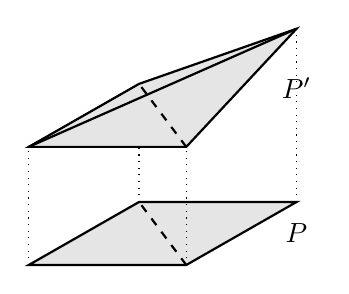
\begin{tikzpicture}
      \draw[thick,fill=black!10] (0,0) -- (2,0) -- (3.4,0.8) -- (1.4,0.8) -- cycle;
      
      \draw[dotted] (0,0) -- (0,1.5);
      \draw[dotted] (2,0) -- (2,1.5);
      \draw[dotted] (3.4,0.8) -- (3.4,3.0);
      \draw[dotted] (1.4,0.8) -- (1.4,2.3);

      \draw[thick,fill=black!10] (0,1.5) -- (2,1.5) -- (3.4,3.0) -- (1.4,2.3) -- cycle;
      \draw[thick,dashed] (2,1.5) -- (1.4,2.3);
      \draw[thick] (0,1.5) -- (3.4,3.0);
      
      \draw[thick,dashed] (2,0) -- (1.4,0.8);
      
      \draw (3.4,0.4) node {$P$};
      \draw (3.4,2.25) node {$P'$};
    \end{tikzpicture}
  \end{center}
  \caption{Triangulate a polytope $P \subset \R^2$ by the projection of the lower envelope of a lifting.}
  \label{fig:triangulation-proof}
\end{figure}
\begin{proof}
  The idea is to lift the vertices of $P$ into $\R^{d+1}$ in such a way
  that essentially every facet of their convex hull $P'$ is a simplex.
  The projection of the lower envelope of $P'$ will then be a triangulation of $P$,
  see Figure~\ref{fig:triangulation-proof}.

  Let us choose $t_1, \ldots, t_n \in \R$ in a manner that is to be described later
  and let $v_i' := (v_i, t_i) \in \R^{d + 1}$.
  Their convex hull
  \[
    P' := \conv\{v_1',\ldots,v_n'\}
  \]
  is a polytope with $\pi(P') = P$,
  where $\pi:\R^{d+1} \to \R^d$ is the projection onto the first $d$ coordinates.

  For every $x \in P$, let
  \[
    \ell(x) := \min\{ t ~:~ (x,t) \in P' \}
  \]
  The point $(x, \ell(x))$ lies in a facet of $P'$
  whose defining inequality $a^Tx + \alpha t \geq \beta$ satisfies $\alpha > 0$.\footnote{This follows
  from the minimality of $\ell(x)$.}
  Let $F_1,\ldots,F_m$ be the set of facets of $P'$ whose defining inequality satisfies $\alpha > 0$
  and let $\Delta_j := \pi(F_j)$.
  We have already shown that
  \[
    P = \bigcup_j \Delta_j
  \]
  Since $\pi$ is injective on the $F_j$, the $\Delta_j$ are full-dimensional
  and for $i \neq j$, $\Delta_i \cap \Delta_j$ is either empty or a face of both $\Delta_i$ and $\Delta_j$,
  since the same property holds for the $F_j$ by basic combinatorics of polyhedra.

  It remains to be shown that the $\Delta_j$ are simplices.
  Standard perturbation arguments show that the $t_i$ can be chosen such that no $d+2$ of the $v_i'$ lie in a hyperplane that does not contain $\ker \pi$.

  Let us show an argument via the polynomial method in detail.
  Consider a subset of $d+1$ affinely independent vertices of $P$, say $v_1, \ldots, v_{d+1}$.
  Their liftings $v_1', \ldots, v_{d+1}'$ will span a hyperplane $H \subset \R^{d+1}$ that does not contain $\ker \pi$.
  Any normal vector $u' = (u,\nu)$ of $H$ satisfies
  \[
    (v_i' - v_{d+1}')^T u' = 0 \text{ for all } i = 1 \ldots d
  \]
  and we can normalize it by requiring
  \[
    \nu = 1.
  \]
  We have obtained a linear system for $u'$ with a square, invertible\footnote{%
  Since we assumed $v_1, \ldots, v_{d+1}$ to be affinely independent, the vectors $v_j - v_{d+1}$ are linearly indpendent.}
  coefficient matrix of the form:
  \[
    \begin{pmatrix}
      v_1^T - v_{d+1}^T & t_1 - t_{d+1} \\
      \vdots & \vdots \\
      v_d^T - v_{d+1}^T & t_d - t_{d+1} \\
      0 & 1
    \end{pmatrix}
  \]
  Using Cramer's rule, we can conclude that each component of $u$ is a multilinear function of the $t_i$.

  Our goal is to choose the $t$ in such a way that every set of $d+1$ affinely independent vertices ends up with a different vector $u$.
  Let
  \[
    t(\lambda) := (\lambda^1, \ldots, \lambda^n)
  \]
  so that every component of every $u$ is a polynomial in $\lambda$.
  Moreover, if we fix two different sets of $d+1$ affinely independent vertices
  and call the corresponding normal vectors $u$ and $\hat u$,
  then the components of the vector $u - \hat u$ are polynomials in $\lambda$,
  at least one of which is non-zero.\footnote{To see this,
  observe that the exponents of the monomials $\lambda^i$ appearing in the polynomials correspond to the indices of vertices.
  Since different sets of vertices are used to define $u$ and $\hat u$,
  they also contain different sets of monomials, which cannot all cancel.}
  That is, there are finitely many values of $\lambda$ for which $u$ and $\hat u$ are equal.

  Taking all pairs of sets of vertices into account,
  there are only finitely many values of $\lambda$
  for which the liftings of two different affinely independent sets of $d+1$ vertices lie in the same hyperplane.
  For all other values of $\lambda$, the facets on the lower envelope of the resulting $P'$ are guaranteed to be simplices.

  Finally, let us remark that the convex hull of a set of points can be computed in polynomial time when the dimension $d$ is fixed,
  and the number of ``bad'' values for $\lambda$ is bounded by $n \binom{n}{d+1}^2$, which is a polynomial in $n$ for fixed $d$.
  Hence all steps of the proof can be made algorithmic, and the resulting algorithm runs in polynomial time
  when the dimension $d$ is fixed.
\end{proof}

\begin{corollary}
  Let $C = \cone\{ u_1, \ldots, u_n \} \subset \R^d$ be a full-dimensional pointed cone.
  Then there exist full-dimensional simplicial cones $C_1, \ldots, C_m \subset \R^d$ spanned by the $u_i$
  such that
  \begin{enumerate}
    \item $C = \bigcup_i C_i$ and
    \item for all $i \neq j$, $C_i \cap C_j$ is a face of both $C_i$ and $C_j$ (possibly the face $\{ 0 \}$).
  \end{enumerate}
  If $C$ is a rational cone, this triangulation can be computed in polynomial time for fixed dimension $d$.
\end{corollary}
\begin{figure}
  \begin{center}
    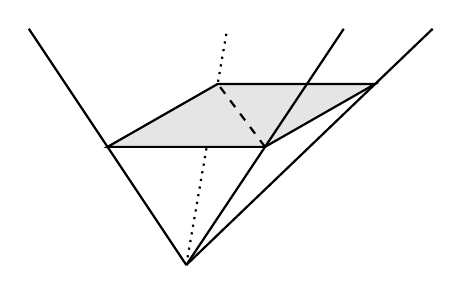
\begin{tikzpicture}
      \draw[thick,dotted] (1,-1.5) -- (1.52,1.5);

      \draw[thick,fill=black!10] (0,0) -- (2,0) -- (3.4,0.8) -- (1.4,0.8) -- cycle;
      \draw[thick,dashed] (2,0) -- (1.4,0.8);

      \draw[thick] (1,-1.5) -- (-1,1.5);
      \draw[thick] (1,-1.5) -- (3,1.5);
      \draw[thick] (1,-1.5) -- (4.13,1.5);
    \end{tikzpicture}
  \end{center}
  \caption{The triangulation of a pointed cone can be obtained from a triangulation of its so-called vertex figure.}
  \label{fig:triangulation-cone}
\end{figure}
\begin{proof}
  Since $C$ is pointed,
  there is an inequality $a^T x \leq 0$ defining its vertex $0$.\footnote{%
  That is, $a^Tx \leq 0$ is valid for $C$ and $a^Tx < 0$ for all $x \in C \setminus \{ 0 \}$.}
  Let $P := C \cap \{ a^Tx = -1 \}$
  and let $\Delta_1, \ldots, \Delta_n$ be its triangulation by Theorem~\ref{thm:polytope-triangulation},
  see Figure~\ref{fig:triangulation-cone}.
  Then the $C_i := \cone \Delta_i$ satisfy the desired properties.
\end{proof}




\section{The algebra of polyhedra}

Given a triangulation of a cone $C$ into simplicial cones $C_1, \ldots, C_n$,
it seems natural to express the generating function $f(C;x)$ as
the sum of the generating functions $f(C_i;x)$.
Note, however, that integer points on lower-dimensional cones that arise from intersections $C_i \cap C_j$
will be counted multiple cones.
The generating functions corresponding to those lower dimensional cones must then be subtracted,
but then points that have been subtracted too often must be added again, and so on.
In this section, we will put such computations on a rigorous foundation.

\begin{definition}
  We denote
  \begin{enumerate}[(a)]
    \item by $\cP^d$ the set of rational polyhedra in $\R^d$,
    \item by $\cP_0^d \subset \cP^d$ the set of rational polyhedra that contain lines,
    \item by $\cP_v^d \subset \cP^d$ the set of rational polyhedra that do not contain lines (i.e., polyhedra with vertices aka pointed polyhedra),
    \item by $\cP_b^d \subset \cP^d$ the set of bounded rational polyhedra, and
    \item by $\cP_\ell^d \subset \cP^d$ the set of rational polyhedra that is not full-dimensional.
  \end{enumerate}
\end{definition}
The relationships between those families of polyhedra are as follows:
\begin{center}
  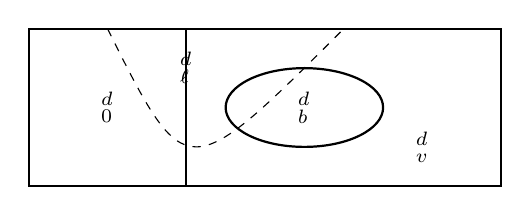
\begin{tikzpicture}
    \draw[thick] (0,0) rectangle (6,2);
    \draw[thick] (2,0) rectangle (2,2);
    \draw (1,1) node {$\cP_0^d$};
    \draw (5,0.5) node {$\cP_v^d$};
    \draw[thick] (3.5,1) ellipse[x radius=1cm,y radius=0.5cm] node {$\cP_b^d$};
    \draw[dashed] (1,2) .. controls (2,0) .. (4,2);
    \draw (2,1.5) node {$\cP_\ell^d$};
  \end{tikzpicture}
\end{center}

\begin{definition}
  Let $P \in \cP^d$.
  The \emph{indicator} or \emph{characteristic} function of $P$ is denoted by $[P] = \chi_P : \R^d \to \R$,
  where
  \[
    [P](x) := \begin{cases}
                1 & x \in P \\
                0 & x \not\in P
              \end{cases}
  \]
  Then $\R \cP^d$ is the sub-vector space of the space of all functions
  that is generated by $\{ [P] : P \in \cP^d \}$.
  The vector spaces $\R \cP_0^d$ etc. are defined analogously.
\end{definition}

\begin{lemma}[Inclusion-exclusion formula]
  \label{lemma:inclusion-exclusion}
  Let $P_1, \ldots, P_m \in \cP^d$.
  Then
  $[A_1 \cup \dots \cup A_m] = \sum_{\emptyset \neq I \subseteq [m]} (-1)^{|I| - 1} [\bigcap_{i \in I} A_i]$.
\end{lemma}
\begin{proof}
  Left as an exercise.
\end{proof}

\begin{lemma}
  \label{lemma:generating-functions-linear-as-series}
  Let $R := \R[[x_1,\ldots,x_d,x_1^{-1},\ldots,x_d^{-d}]]$ be the vector space of formal power series in $d$ variables.\footnote{%
  This is \emph{not} a ring, because multiplication of formal power series with unbounded positive \emph{and} negative exponents is not defined.}
  There exists a unique linear map $F: \R \cP^d \to R$
  such that $F([P]) = f(P;x)$ for all $P \in \cP^d$.
\end{lemma}
\begin{proof}
  If we can show that one such $F$ exists,
  then uniqueness follows immediately because its values are fixed on a generating set of $\R\cP^d$.
  If the $[P]$ for $P \in \cP^d$ were linearly independent,
  then existence of $F$ would be obvious.
  Since they are not, we need to show that our desired values of $F$ are consistent under linear dependencies.

  To be precise, we need to show that for all linear dependencies of the form
  \[
    \sum_{i=1}^n \alpha_i [P_i] = 0
  \]
  one has
  \[
    \sum_{i=1}^n \alpha_i f(P_i; x) = 0,
  \]
  where the equality is in the sense of formal power series.

  The equality of formal power series is defined as the equality of all coefficients.
  That is,
  we need to determine the coefficient $a_p$ of the monomial $x^p$
  for every integer point $p \in \Z^d$.
  In fact,
  \[
    a_p = \sum_{i: p \in P_i} \alpha_i = \left(\sum_{i=1}^n \alpha_i [P_i] \right)(p) = 0 \text{ for all } p \in \Z^d,
  \]
  which completes the proof.
\end{proof}

\begin{corollary}
  \label{corollary:cone-triangulation-series}
  Let $C \in \cP^d$ be a pointed cone with triangulation $C_1, \ldots, C_n \in \cP^d$.
  Then
  \[
    f(C;x) = \sum_{\emptyset \neq I \subseteq [n]} (-1)^{|I| - 1} f(\bigcap_{i \in I} C_i; x)
  \]
  where the equality is understood as equality of formal power series.
\end{corollary}
\begin{proof}
  Follows from Lemmas~\ref{lemma:inclusion-exclusion} and~\ref{lemma:generating-functions-linear-as-series}.
\end{proof}

The sum in Corollary~\ref{corollary:cone-triangulation-series} typically contains
many index sets $I$ for which the intersection $\bigcap_{i \in I} C_i$ is trivial,
i.e., equal to $\{ 0 \}$.
Using tools that we will develop later, it turns out that those summands can be ignored.
Showing this is left as an exercise.

While Lemma~\ref{lemma:generating-functions-linear-as-series}
rigorously justifies computations with power series $f(P;x)$,
we really want an anologous statement for rational functions.
This is not immediate because, as we have seen in Section~\ref{sec:simple-example-generating-functions},
the series $f(P;x)$ converges nowhere for $P \in \cP_0^d$,
and so it is not clear what rational function to assign to such polyhedra.
However, it turns out that assigning rational functions to \emph{pointed} polyhedra is sufficient:

\begin{lemma}
  \label{lemma:algebra-generated-by-pointed}
  $\R \cP^d = \R\cP_v^d$.
\end{lemma}
\begin{proof}
  The inclusion from right to left is immediate.
  We need to show that $[P] \in \R\cP_v^d$ for all $P \in \cP_0^d$;
  the inclusion from left to right then follows by linearity.

  Let $Q_1, \ldots, Q_n \in \cP_v^d$ and $\varepsilon_1, \ldots, \varepsilon_n \in \R$ such that
  \[
    [\R^d] = \sum_{i=1}^n \varepsilon_i [Q_i]
  \]
  One can obtain such an equation by applying the inclusion-exclusion formula to the orthants of $\R^d$.
  We then observe that pointwise multiplication of indicator functions of polyhedra
  corresponds to taking intersections, and compute:
  \[
    [P] = [\R^d] \cdot [P] = \sum_{i=1}^n \varepsilon_i [Q_i] \cdot [P] = \sum_{i=1}^n \varepsilon_i [Q_i \cap P] \in \R\cP_v^d,
  \]
  since the subset $Q_i \cap P$ of the pointed polyhedron $Q_i$ is pointed as well.
\end{proof}
\begin{figure}
  \begin{center}
    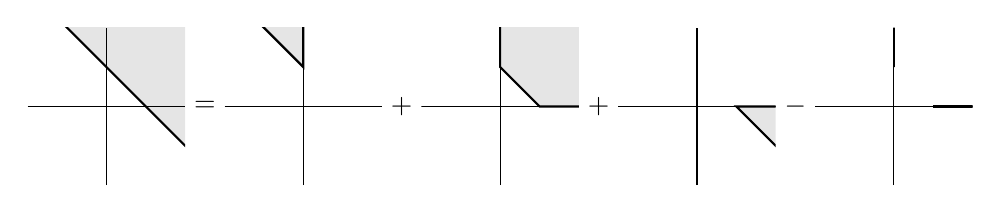
\begin{tikzpicture}
      \begin{scope}
        \clip (-1,-1) rectangle (1,1);

        \draw[thick,fill=black!10] (-1,1.5) -- (1.5,-1) -- (1.5,1.5) -- cycle;
        \draw (-1,0) -- (1,0);
        \draw (0,-1) -- (0,1);
      \end{scope}

      \draw (1.25,0) node {$=$};

      \begin{scope}[xshift=2.5cm]
        \clip (-1,-1) rectangle (1,1);

        \draw[thick,fill=black!10] (-1,1.5) -- (0,0.5) -- (0,1.5) -- cycle;
        \draw (-1,0) -- (1,0);
        \draw (0,-1) -- (0,1);
      \end{scope}

      \draw (3.75,0) node {$+$};

      \begin{scope}[xshift=5cm]
        \clip (-1,-1) rectangle (1,1);

        \draw[thick,fill=black!10] (0,1.5) -- (0,0.5) -- (0.5,0) -- (1.5,0) -- (1.5,1.5) -- cycle;
        \draw (-1,0) -- (1,0);
        \draw (0,-1) -- (0,1);
      \end{scope}

      \draw (6.25,0) node {$+$};

      \begin{scope}[xshift=7.5cm]
        \clip (-1,-1) rectangle (1,1);

        \draw[thick,fill=black!10] (1.5,-1) -- (0.5,0) -- (1.5,0) -- cycle;
        \draw (-1,0) -- (1,0);
        \draw (0,-1) -- (0,1);
      \end{scope}

      \draw (8.75,0) node {$-$};

      \begin{scope}[xshift=10cm]
        \clip (-1,-1) rectangle (1,1);

        \draw[thick,fill=black!10] (0,0.5) -- (0,1) -- cycle;
        \draw[thick,fill=black!10] (0.5,0) -- (1,0) -- cycle;
        \draw (-1,0) -- (1,0);
        \draw (0,-1) -- (0,1);
      \end{scope}
    \end{tikzpicture}%
  \end{center}
  \caption{An illustration of the proof of Lemma~\ref{lemma:algebra-generated-by-pointed}.}
  \label{fig:algebra-generated-by-pointed}
\end{figure}




\section{Rational generating functions of polyhedra}





\section*{Exercises}

\begin{enumerate}
  \item Show Lemma~\ref{lemma:cone-polars}.

  \item Show Lemma~\ref{lemma:simplicial-cone-polars}.

  \item Show the inclusion-exclusion formula (Lemma~\ref{lemma:inclusion-exclusion}).

  \item Show the remark after Corollary~\ref{corollary:cone-triangulation-series}:
    In the expression
    \[
      f(C;x) = \sum_{\emptyset \neq I \subseteq [n]} (-1)^{|I| - 1} f(\bigcap_{i \in I} C_i; x)
    \]
    for a triangulation of a pointed cone $C$,
    the trivial summands on the right hand side add up to $0$.

    \emph{Hint:} You can apply the Euler characteristic to the inclusion-exclusion formula applied to the vertex figure of the triangulation.
\end{enumerate}
